 \section{Architektura}
 Cílem této práce je vytvoření programu, který bude schopen detekovat anomální provoz v~IoT sítích. 
 Vzhledem k~hardwarovým omezením, které můžou na IoT branách nastat, je architektura navržena tak, aby
 měla co nejmenší nároky na dostupné prostředky. Schéma nasazení detekčního systému se nachází
 na Obrázku \ref{obr.deploy-arch}
 
 \begin{figure}[ht]
   \begin{center}
   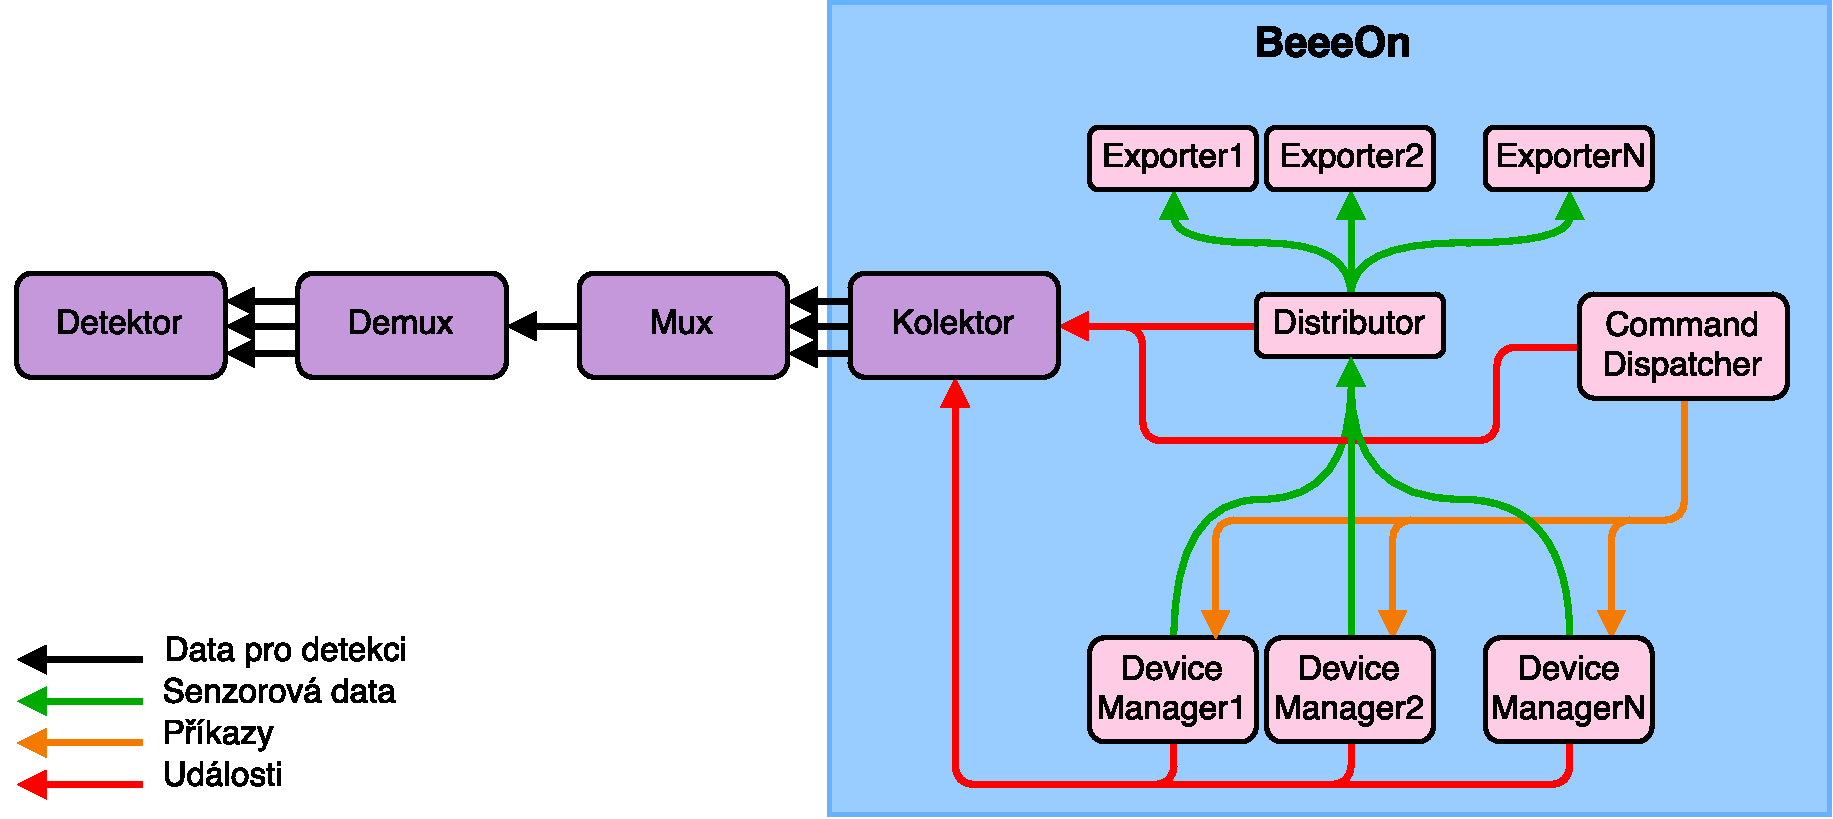
\includegraphics[scale=0.52]{pictures/deploy-arch}
   \caption{Architektura detekčního systému}
   \label{obr.deploy-arch}
   \end{center}
   \end{figure}
 
 Implementace BeeeOn brány obsahuje pro zpracování senzorových dat následující komponenty:
 \begin{itemize}
  \item \textbf{DeviceManager}:
    komponenta definovaná pro každý senzorový protokol, která implementuje veškerou komunikaci
    a zpracování dat
    
  \item \textbf{Distributor}:  
  přijímá data od \textit{DeviceManageru}, která následně předává příslušnému \textit{Exporteru}
  
  \item \textbf{Exporter}:
  implementuje protokol, kterým jsou data odesílány z~brány
  
  \item \textbf{CommandDispatcher}:  
  přijímá uživatelské příkazy a distribuuje je cílovým komponentám
  
 \end{itemize}
 
 Každá z~komponent v~BeeeOn bráně navíc využívá návrhový vzor \textit{Observer}, pomocí kterého jsou
 definovány události poskytující informace o~každé komponentě. 
 Tímto způsobem bude vytvořený kolektor získávat data o~provozu, která
 převede do formátu UniRec (Unified Record) a pomocí systému NEMEA je odešle k~analýze.
 
 Exportované informace o~provozu bude přijímat detektor, který následně provede jejich zpracování a 
 vyhodnocení stavu. Všechny vytvořené komponenty určené pro detekci budou používat rozhraní 
 NEMEA. Díky tomu bude možné komponenty flexibilně provozovat na jednom nebo více různých zařízeních.
 Oddělené nasazení je důležité zejména pro brány s~omezenými prostředky, které mohou provádět 
 pouze export dat a o~vyhodnocení se bude starat odlišné zařízení s~dostatečným výkonem. V~případě 
 provozování více bran lze brány používat jako exportéry a veškerá získaná data zpracovávat 
 centrálně. 
 
 Kolektor pro každý typ události vytvoří samostatné výstupní komunikační rozhraní, kterých 
 při reálném provozu může být velké množství. Z~tohoto důvodu  
 bude vytvořen modul \textit{Mux}, který všechna výstupní rozhraní spojí do jednoho společného. 
 Pro zpětné rozdělení na jednotlivé typy událostí bude sloužit modul \textit{Demux}. Tyto moduly budou velmi užitečné
 zejména v~případě, kdy kolektor a detektor budou na rozdílných síťových prvcích, protože údaje 
 o~provozu budou přenášeny přes počítačovou síť a bude vyžadováno zabezpečení všech odchozích komunikačních
 rozhraní. S~využitím \textit{Mux} a \textit{Demux} modulů bude stačit zabezpečit pouze jedno sjednocené rozhraní. 
 
 Výhodou návrhu řešení je flexibilita a modularita. Každá komponenta vždy samostatně pokrývá pouze jednu
 část detekčního systému a díky NEMEA se každá z~nich může nacházet na různých síťových prvcích. Zároveň
 v~případě potřeby lze vytvořit další moduly, které budou rozšiřovat stávající funkcionalitu.
 Podrobnější popis návrhu nově vytvořených komponent detekčního systému se nachází v~následujících sekcích.
 
 \section{Kolektor}
 Úkolem kolektoru bude sběr dostupných dat a jejich odeslání k~následné analýze. Informace
o~provozu budou sbírány z~jednotlivých komponent BeeeOn brány, které jsou zpřístupňovány pomocí 
 návrhového vzoru \textit{Observer}. Z~tohoto důvodu bude kolektor vždy přímou součástí BeeeOn brány. 
 Návrh struktury kolektoru je na Obrázku \ref{obr.modelTrid}
 
 \begin{figure}[ht]
   \begin{center}
   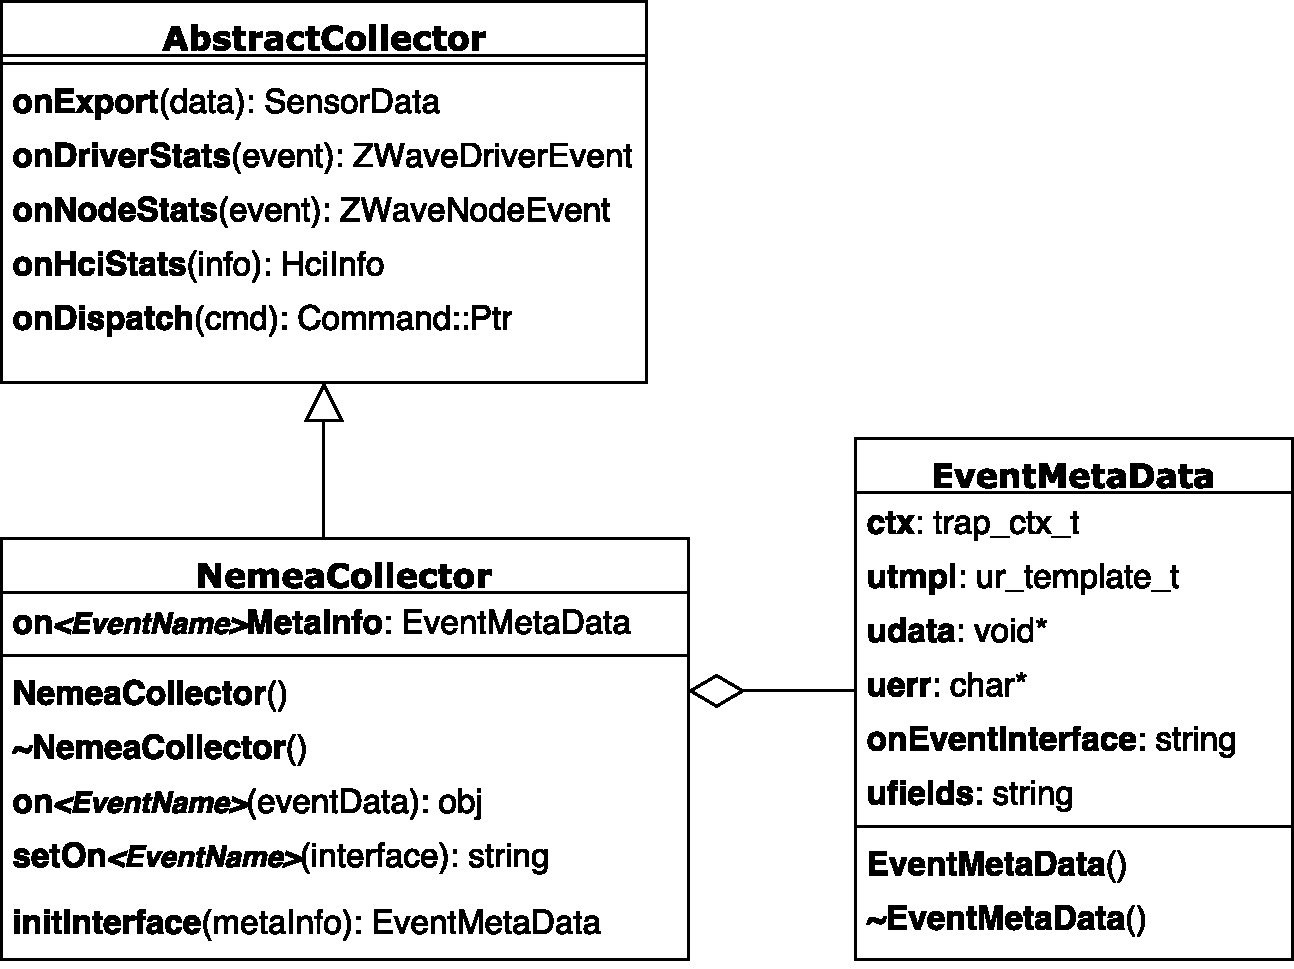
\includegraphics[scale=0.5]{pictures/modelTrid}
   \caption{Návrh kolektoru provozních dat}
   \label{obr.modelTrid}
   \end{center}
   \end{figure}
 
 \textit{AbstractCollector}, je třída vytvořená v~projektu BeeeOn, které shromažďuje všechny dostupné
 typy událostí.
 V~současné době jsou k~dispozici následující události:
 \begin{itemize}
  \item \textbf{onExport}:
   reprezentuje hodnoty dat přicházejících ze senzorů, která jsou odeslána vždy po jejich příjmu
   
  \item \textbf{onDriverStats}:
   v~pravidelných intervalech generuje statistiky o~Z-Wave sítí dostupné na komunikačním 
   rozhraní
   
  \item \textbf{onNodeStats}:
   periodicky získává informace o~jednotlivých prvcích umístěných uvnitř jedné Z-Wave sítě, které jsou dostupné pomocí
   knihovny OpenZWave
   
  \item \textbf{onHciStats}:
   v~definovaných intervalech získává z~komunikačního rozhraní pro BLE statistiky o~provozu
   sítě
  
  \item \textbf{onDispatch}:
  umožňuje získávat zadané uživatelské příkazy
 \end{itemize}

 Vytvořený kolektor je reprezentován třídou \textit{NemeaCollector}, která je potomkem třídy
 \textit{AbstractCollector} a bude implementovat všechny její členské funkce pro zachytávání událostí. Pro každou 
 členskou funkci  bude vytvořen setter, který při spuštění brány provede počáteční nastavení
 parametrů pro obsluhu dané 
 události. Vstupním parametrem bude řetězec určující název výstupního rozhraní, který bude
 specifikovaný
v~konfiguračním souboru BeeeOn brány. Po nastavení počátečních parametrů jako je název výstupního
 rozhraní a seznam UniRec polí se zavolá členská funkce \textit{initInterface()}, jejímž cílem bude inicializace
 veškerých struktur vyžadovaných NEMEA frameworkem.
 Jako vstupní parametr bude přijímán objekt \textit{EventMetaData} udržující veškeré informace potřebné 
 k~odesílání získaných dat.
 
 Instance objektu \textit{EventMetaData} bude vytvořena jako členská proměnná třídy \textit{NemeaCollector}
 pro každou členskou funkci události. Díky tomu bude možné každou událost zpracovávat nezávisle dle
 definovaných parametrů.
 
 Definované konstruktory a destruktory budou sloužit jen pro vytvoření a~destrukci potřebných 
 struktur. Tímto bude zajištěn programovací idiom RAII (Resource Acquisition Is Initialization).
 
 Veškeré odesílané údaje budou rozšířeny o~časovou značku a číselný identifikátor, aby mohl detektor
 přesně určit původ případné anomálie.
 
 \newpage
 \section{Detektor}
 Detektor bude hlavní komponentou celého řešení, protože bude vyhodnocovat získaná data. Vzhledem
 k~zadaným požadavkům musí být návrh proveden tak, aby bylo umožněno budoucí rozšiřování. Návrh 
 architektury je zobrazen na Obrázku \ref{obr.detektor}
 \begin{figure}[ht]
   \begin{center}
   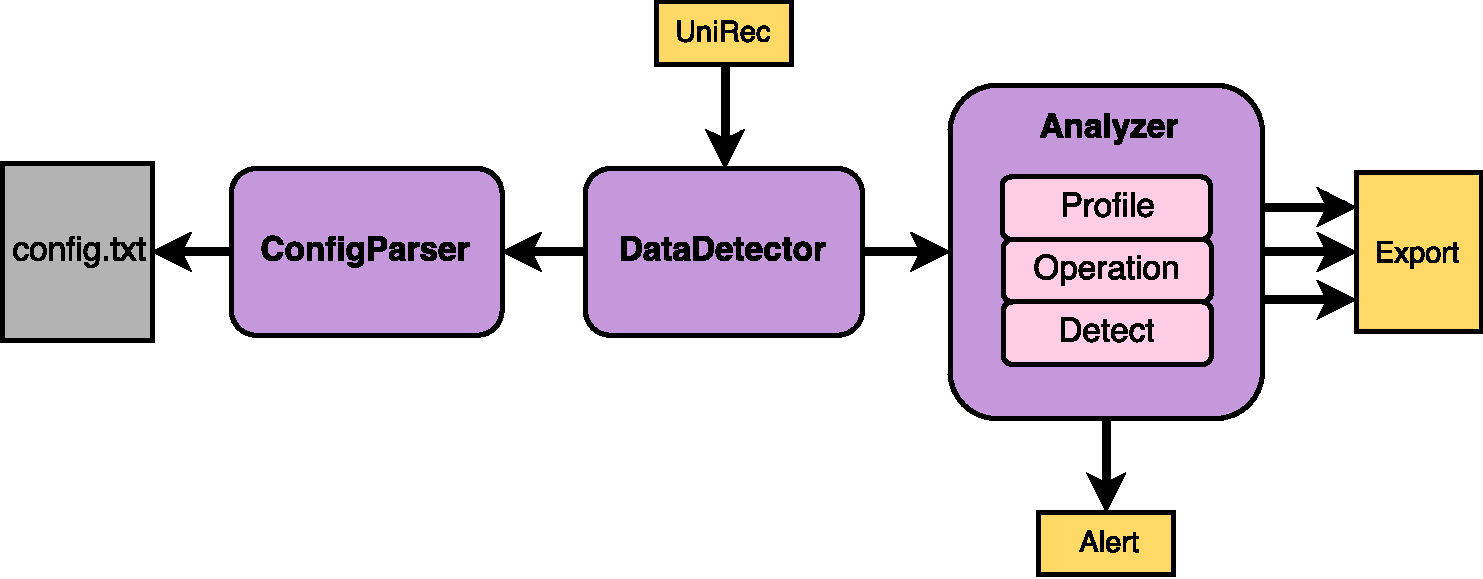
\includegraphics[scale=0.6]{pictures/detektor-arch}
   \caption{Architektura detektoru}
   \label{obr.detektor}
   \end{center}
   \end{figure}

 Komponenta \textit{DataDetector} bude mít jedno vstupní rozhraní, kterým bude přijímat data z~kolektoru.
 V~případě potřeby
 zpracování více událostí z~kolektoru lze využít již existující NEMEA modul \textit{Merger}, který
 dokáže sloučit více vstupů do jednoho konsolidovaného výstupu. 
 
 Dále se v~rámci třídy \textit{DataDetector} bude volat \textit{ConfigParser}, který bude mít na starosti zpracování 
 konfiguračního souboru. Konfigurační soubor bude obsahovat seznam parametrů pro každé UniRec pole,
 na základě kterých bude vytvořena instance třídy \textit{Analyzer} pro analýzu dat. 
 
 Po provedení inicializace všech modulů bude \textit{DataDetector} pouze přijímat data z~kolektoru a 
 předávat je ke zpracování komponentě \textit{Analyzer}. Tato komponenta bude obsahovat
 tři hlavní části:
 \begin{itemize}
  \item \textbf{Profile}
  
  Bude obsahovat členské funkce, které se budou starat o~připravení profilu sítě. 
  Vytvořený profil bude složen z: průměru, klouzavého průměru, klouzavého
  rozptylu a klouzavého mediánu \ref{profileDef}.
  Tyto hodnoty budou následně použity při porovnávání s~aktuálním provozem v~rámci detekčních
  metod. V~případě potřeby bude možné profil rozšířit o~další hodnoty.
  
   \item \textbf{Operation}
  
  Cílem této části bude udržování veškerých použitých struktur. Bude se jednat o~struktury 
  pro konfiguraci, zpracovávaná data a odesílání získaných výsledků. Odesílat lze informaci
o~nalezené hrozbě, pro kterou se používá jedno společné rozhraní, nebo pravidelně exportovat
  definované části aktuálního profilu sítě pro účely dalšího zpracování. Obsahem zprávy s~nalezeným
  incidentem bude: ID zdroje dat, časové razítko, hodnota anomálie, hodnota položky vzorového profilu, 
  název položky vzorového profilu, název UniRec klíče a popis anomálie. V~rámci pravidelného exportu
  se budou odesílat jen definované číselné položky z~aktuálního profilu.
  
  \item \textbf{Detect}
  
  Bude sdružovat všechny členské funkce určené pro detekci anomálií v~získaných datech. 
  Každá členská funkce bude reprezentovat jedno kritérium a bude možné budoucí rozšíření o~další
  potřebné metody. V rámci vytvořeného řešení budou dostupná kritéria pro detekci: neočekávaného
  růstu, překročení vymezených hodnot a porušení periodicity \ref{detectMethods}.
  
 \end{itemize}

 Díky konfiguraci organizované po jednotlivých UniRec polích bude možné nastavit chování výše
 popsaných částí nezávisle pro každé pole.
 
 \subsection{Konfigurace modulu} \label{config_file}
 Jedním z~funkčních požadavků je možnost konfigurace způsobu detekce, která se tak bude moci přizpůsobit 
 cílovým podmínkám. Každá instance detektoru bude mít jeden konfigurační soubor, který bude 
 popisovat jednotlivá UniRec pole určená pro analýzu.
 
 Konfigurace bude v~textové podobě ve formátu klíč a seznam hodnot. Textová podoba je velmi vhodná pro 
 fázi ladění a vývoje nástroje, protože jsou možné manuální úpravy. Cílem ovšem je generovat 
 konfiguraci pomocí externího nástroje, který by mohl být součástí řídící vrstvy IoT brány. 
 
 Klíčem bude vždy název UniRec pole, který se bude nacházet v~příchozích datech. Za tímto klíčem
 se může nacházet volitelně číselný identifikátor senzoru, který se musí shodovat
s~identifikátorem odesílaným z~kolektoru. Důsledkem toho bude možnost detekční parametry
 definovat i pro jednotlivá zařízení pokud se jich pod jedním UniRec názvem bude nacházet 
 více. V~případě neuvedení identifikátoru se jako výchozí hodnota použije číslo nula.
 Takto definovaná hlavička bude oddělena dvojtečkou, za kterou bude sekvence parametrů
 oddělených středníkem. Každý nový záznam s~popisem přicházejících dat
 se bude nacházet na samostatném řádku. Řádky prázdné a začínající znakem \textit{\#} budou
 považovány za komentář. 
 
 
 Definované parametry budou rozděleny do následujících hlavních skupin:
 \begin{itemize}
  \item \textbf{General} 
  
  Tato skupina bude obsahovat obecné volby pro definování časové řady. Pomocí číselných parametrů 
  bude možné určit velikost řady, délku učící fáze, během které bude vytvořen profil sítě a její délka
  musí být stejná nebo delší než velikost časové řady, a rozsah ignorovací části, která bude vhodná
  k~odfiltrování počáteční výměny zpráv při navazování spojení. 
  
  Dalším parametrem bude způsob 
  ukládání dat do časové řady. K~dispozici budou dva režimy. Prvním z~nich bude \textit{simple},
  který přijatou
  hodnotu pouze uloží. Druhý bude \textit{delta}, který bude vkládat rozdíly dvou po
  sobě jdoucích hodnot. 
  Toto bude vhodné zejména u~časových značek nebo počtu odeslaných zpráv, protože bude vhodnější 
  udržovat jednotlivé přírůstky než pouhé absolutní hodnoty. 
  
  Poslední volbou budou číselné hodnoty určující rozmezí mezi pravidelnými kontrolami
  přijetí a změny dat a 
  číselný parametr definující periodu pro exportování vybraných parametrů. Nastavení těchto položek
  bude volitelné. Jejich nepoužití bude označeno znakem \textit{-}.
  
  \item \textbf{Profile}
  
  Zápis této skupiny bude identifikovaný klíčovým slovem \textit{profile}, který má uvnitř kulatých závorek 
  vyjmenované jednotlivé položky, které budou součástí vytvořeného profilu. Ve vytvořeném řešení 
  budou k~dispozici následující volby: \textit{average} (průměr), \textit{moving\_variance} (klouzavý rozptyl), 
  \textit{moving\_median} (klouzavý medián) a \textit{moving\_average} (klouzavý průměr) \ref{profileDef}.
  Součástí profilu bude vždy alespoň
  jedna položka. Použité části a jejich počet bude vždy záviset na uživateli.
  
  \item \textbf{Profile Values}
  
  Pro každou položku definovanou v~rámci profilu musí být uveden seznam jejich detekčních parametrů.
  Zápis bude probíhat pomocí klíčového slova z~profilu, které bude mít jednotlivé hodnoty 
  specifikované uvnitř kulatých závorek. Zde bude možné určit minimální nebo maximální soft a~hard
  limity, kterých daná položka aktuálního profilu může dosahovat. Pro soft limit bude dále možné 
  určit povolenou délku, po kterou může být nastavená hranice překročena (grace period). 
  
  Dalšími parametry budou číselné hodnoty určující meze pro minimální a maximální velikost 
  změny sledované položky ve srovnání s~vzorovým profilem. Všechny ostatní argumenty nebudou mít
  žádný význam pro konfiguraci, ale 
  budou sloužit jako proměnné pro ukládání dočasných hodnot.
  
  Zadání veškerých hodnot nebude nutné a tudíž bude záležet na uživateli, které způsoby detekce 
  bude chtít využít. V~případě nedefinování některého parametru bude zapsán znak \textit{-}.
  Na základě nastavených hodnot se budou volat příslušné detekční metody.
  
  \item \textbf{Export}
  
  Poslední nastavitelnou možností bude export vybraných dat z~profilu. Zápis bude probíhat pomocí 
  klíčového slova \textit{export}, který v~kulatých závorkách bude mít seznam položek z~profilu. Zároveň 
  v~případě využití této možnosti bude nutné ve skupině \textit{general} určit časovou periodu
  odesílání.
  Názvy výstupních \textit{libtrap} rozhraní
  budou odvozené od klíčů, které se nacházejí před dvojtečkou v~konfiguraci.
  
 \end{itemize}

 Příklad záznamu s~konfigurací je na Obrázku \ref{obr.config}. Jednotlivé barvy označují 
 výše definované skupiny. 
 
 Nastavení formou
 souboru bude jedninou volbou pro přizpůsobení detekce. Dále při 
 spuštění programu bude očekáván povinný přepínač \textit{-i}, který je vyžadován knihovnou 
 \textit{libtrap} a bude definovat název vstupního
 rozhraní pro příchozí data a název výstupního rozhraní pro detekované incidenty. Jako nepovinný přepínač
 bude možná zadat \textit{-v}, jehož výsledkem bude zapnutí ladících výpisů. Tato volba bude umožňovat 
 až tři úrovně podrobnosti výpisů. Tyto úrovně budou určeny počtem znaků \textit{v}.
 
   \begin{figure}[ht]
   \begin{center}
   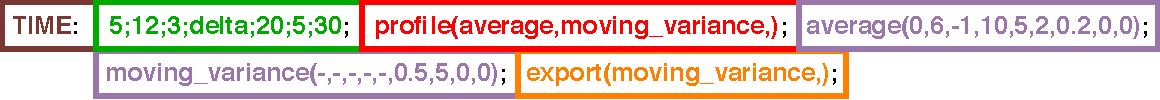
\includegraphics[scale=0.6]{pictures/config-file-frame-mod}
   \caption{Popis konfiguračních parametrů pro jeden záznam}
   \label{obr.config}
   \end{center}
   \end{figure}
 
 \subsection{Použité struktury}
 Velmi důležitou částí návrhu bude určení formátu použitých struktur, které budou udržovat veškeré 
 údaje nutné pro analýzu. V~rámci detektoru bude potřeba udržovat informace pro následující
 položky:
  \begin{itemize}
   \item \textbf{Konfigurační parametry} \label{configParam}
   
   Tato struktura bude hierarchicky ukládat veškeré hodnoty z~konfiguračního souboru
   a také údaje nutné k~provedení analýzy. V~první úrovni se budou nacházet názvy jednotlivých 
   UniRec polí, které budou fungovat jako klíče. V~druhé vrstvě bude seznam identifikátorů 
   odlišující senzory skryté pod stejným klíčem.
   Třetí úroveň bude vždy obsahovat stejnou 
   sekvenci podklíčů, které budou určovat typ uchovávaných dat. Bude se jednat o~jednotlivé 
   skupiny z~konfiguračního souboru \ref{config_file}, které budou označeny stejnojmennými
   identifikátory. Hodnotou těchto skupin budou specifikované parametry detekce dle zapsané
   konfigurace. Dále zde budou podklíče s~názvem \textit{metaProfile} a \textit{metaData},
   které budou mít
   stejné položky. Tyto položky budou obsahovat vypočtené údaje z~příslušné časové řady
   a zároveň budou umožňovat ukládání dat, která budou nutná k~provedení výpočtu 
   a vkládání nových prvků. Rozdíl mezi \textit{metaProfile} a \textit{metaData} bude typ profilu,
   pro který budou určeny. Podklíč \textit{metaProfile} bude uchovávat údaje pro vzorový profil,
   který bude vytvořen během učící fáze a bude sloužit pro určení anomálie. Zatímco 
   hodnoty v~\textit{metaData} budou vztaženy k~aktuálnímu profilu sítě, který se mění s~každým
   nový prvkem v~časové řadě.

   \item \textbf{Senzorová data}
   
   Cílem této struktury bude hierarchicky ukládat přicházející data z~kolektoru do časových řad. 
   V~první úrovni se jako v~předchozím případě budou nacházet názvy jednotlivých UniRec polí. 
   Protože jedno UniRec pole může reprezentovat data z~více různých senzorů nebo bran, tak se na 
   další úrovni nachází identifikátor zdroje dat. Předpokládá se, že každá použitá brána a senzor 
   bude mít v~rámci jedné instance detektoru unikátní identifikátory. Na třetí úrovni se bude vyskytovat 
   definovaná časová řada, která uloží data podle zadané konfigurace.
   
   \item \textbf{Nastavení pro export} 
   
   Parametry pro export budou uchovány ve struktuře s~formátem klíč a~hodnota. Klíčem bude 
   pořadové číslo výstupního komunikačního rozhraní, které bude odpovídat konkrétnímu UniRec poli. Hodnotou 
   bude sekvence názvů určující jednotlivé části profilu, které se budou exportovat. Tyto názvy
   budou definované v~konfiguračním souboru. 
   
  \end{itemize}

 
 \subsection{Způsob analýzy}
 Veškerá analýza dat bude prováděna pomocí časových řad, které jsou vhodné pro statistický typ 
 dat a metodu detekce anomálií. Zároveň parametry řad budou nastavitelné, aby bylo možné se přizpůsobit
 pro danou datovou položku, ale i cílovou bránu, na které může být spuštěný detektor. Způsob 
 zpracování dat lze rozdělit do následujících fází:
  \begin{itemize}
   \item \textbf{Inicializace}
   
   V~rámci této sekce budou načteny všechny konfigurační položky a inicializovány veškeré struktury
   nutné pro běh celého řešení. Následně bude program očekávat příchozí data na jediném vstupním
   rozhraní.
   
   \item \textbf{Učení}
   
   Po prvotním přijetí hodnot z~kolektoru bude probíhat stanovení vzorového profilu sítě pro položky,
   které budou popsány v~konfiguračním souboru. V~rámci
   této periody se do časové řady budou vkládat přicházející data a s~každým novým prvkem 
   bude prováděn výpočet všech částí profilu, které budou určeny konfiguračním souborem.
   Pokud bude délka učící fáze delší než velikost 
   časové řady, tak budou všechny prvky posunuty, a tím nejstarší z~nich uvolní místo pro nový.
    \newpage
   \item \textbf{Detekce}
   
   Jakmile bude stanoven vzorový profil sítě, tak se zahájí analýza provozu pro určení anomálií.
   S~každým nový příchozím prvkem bude z~příslušné časové řady vypočítáván aktuální profil sítě,
   který budou používat detekční metody. Dostupné metody jsou popsány v~\ref{detectMethods}.
   
  
   \item \textbf{Vyhodnocení}
   
   Výsledky detekčních metod budou sloužit k~určení stavu provozu. Pokud budou data vyhodnocena jako
   bezpečná, tak nebude provedena žádná akce a přejde se k~obsluze další přijaté hodnoty z~kolektoru.
   V~případě nalezení anomálie se vytvoří zpráva s~informacemi popisující událost, která bude 
   odeslána výstupním rozhraním určeném pro detekované hrozby.   
  \end{itemize}
  
  \newpage
 \section{Multiplexor a demultiplexor}
 Hlavním cílem těchto dvou modulů bude ulehčit nasazení analýzy dat v~případě fyzicky odděleného
 kolektoru a detektoru. Bez použití těchto modulů bude nutné na kolektoru zabezpečit přenos dat
 z~každého výstupního komunikačního rozhraní, což zvýší nároky na výkon brány a zároveň bude vyžadováno
 více konfigurace. Díky multiplexoru bude možné spojit několik různých \textit{libtrap} 
 rozhraní do jednoho, které lze demultiplexorem zase zpětně rozdělit na cílovém zařízení.
 Tímto bude pro export dat z~brány nutné zabezpečit pouze jedno rozhraní.

 Multiplexor bude vícevláknový NEMEA modul, kde každé vlákno bude naslouchat na specifikovaném
 vstupním rozhraní. Po přijetí nového formátu dat se nejprve odešle \textit{hello} zpráva, která
 bude obsahovat popis nového formátu. V~případě přijetí zprávy se stejným formátem bude tato 
 zpráva rovnou přeposlána. Oba typy zpráv budou mít stejnou hlavičku s~položkami: 
 identifikátor zprávy, 
 číslo vstupního rozhraní a typ formátu. Ostatní data nutná pro přenos budou zapouzdřena
v~záhlaví. Díky stejnému formátu zprávy bude možné veškerá data zasílat jedním společným rozhraním.
 
 Demultiplexor bude jednovláknový modul, který bude přijímat na jednom vstupním rozhraní zprávy
 od multiplexoru. Po přijetí dat provede jejich zpracování a na základě identifikátoru 
 provede příslušnou akci. V~případě typu \textit{hello} se upraví nový formát pro specifikované 
 komunikační rozhraní. V~druhém případě se jen přepošlou přijatá data příslušným výstupem.
 
 \newpage
 \section{Scénáře útoků} \label{utoky}
 Na základě vypracované analýzy a provedených experimentů s~protokoly Z-Wave a BLE byly navrženy
 následující scénáře, které mohou v~reálném provozování IoT sítě nastat a identifikovat zneužití
 zranitelnosti díky vzniku anomálního provozu. V~popsaných scénářích se bude vyskytovat jen nezbytně
 nutná množina informací, kterou bude nutné sledovat. Popis všech dostupných dat se nachází
 v~příloze \ref{sensorData}.
 
   \begin{enumerate}
    \item \textbf{Periodicita dat}
    
    Velké množství koncových prvků v~senzorové vrstvě se chová periodicky. Kvůli úspoře napájecí
    energie jsou senzory často v~režimu spánku a jen v~určitých časových okamžicích se probudí, 
    aby odeslaly potřebné údaje. Dále lze využít pravidelnosti BeeeOn brány, která statistiky
    o~jednotlivých komunikačních protokolech exportuje ve stálých časových intervalech. 
    
    Tento scénář se bude soustředit na analýzu času příchozích dat, aby určil případné
    nestandardní chování. Díky tomu bude možné odhalit vzniklé problémy na bráně, které vedou
k~nepravidelnému odesílání informací o~provozu. V~případě, že bude použito čidlo s~periodickým 
    chodem, bude možné zjistit změnu jeho chování nebo jeho úplné odpojení.
    
    Určení času příchozích dat bude snadné, protože každý přijatý záznam bude obsahovat 
    datovou položku s~časovou známkou.
    
    \item \textbf{Množství přenášených zpráv} \label{dos}
    
    Velkou hrozbou, kterou představuje nástup IoT jsou nejrůznější varianty DoS útoků. Konkrétně
    nejobávanějším typem je pravděpodobně zahlcení cílové komunikační linky, protože v~síti bude 
    dostupné obrovské množství prvků, které útočník může v~případě napadení využít. Zároveň
    nejlepším místem, kde tyto útoky zastavit, je zdroj jejich vzniku. Tento scénář může také 
    identifikovat připojení dalšího zařízení.
        
    Cílem bude identifikovat neobvyklý nárůst nebo pokles přenášených dat v~porovnání 
    s~naučeným vzorovým profilem sítě. 
    
    Výhodou jsou Z-Wave sítě, protože nabízí statistiky pro celou síť i pro jednotlivé senzory. 
    Položka \textit{SOAFCount} určuje celkový počet detekovaných zpráv ve vytvořené topologii.
    Při analýze
    jednotlivých čidel bude možné sledovat čítače \textit{receivedCount} a \textit{sentCount}.
    První čítač reprezentuje počet zpráv od konkrétního
    čidla, který byl přijat na bráně. Druhá hodnota určuje počet odeslaných zpráv danému
    senzoru.
    
    BLE nabízí pouze celkové informace, kterých navíc není tolik. V~rámci této detekce bude vhodné 
    použít položky \textit{rxBytes} a \textit{txBytes}, které odpovídají počtu přijatých
    a odeslaných bytů.
    
    \item \textbf{Limity senzorových hodnot}
    
    Tento případ užití se zaměřuje přímo na získávané hodnoty z~čidel. Pro tyto hodnoty se většinou
    dá určit jejich minimální a maximální hodnota s~rychlostí růstu. Pokud se vývoj hodnot nebude 
    shodovat s~očekáváním, může to znamenat poruchu čidla nebo neočekávanou událost, jejíž příčinou 
    může být i útok.
    
    Možnost této detekce bude záviset na události \textit{onExport}, která exportuje všechna
    získaná data nezávisle na použitém protokolu.
    
    \item \textbf{Kvalita přenosového kanálu} \label{kvalita}
    
    Zejména u~bezdrátových komunikačních protokolů je velmi důležitá kvalita přenosového kanálu,
    který může být případným útočníkem zarušen. V~situaci, že tento typ útoku nastane, budou 
    detekční metody očekávat zhoršení statistik komunikace. 
    
    Knihovna OpenZWave nabízí pro každé čidlo informace o~hodnotě RTT (Round-Trip Time). Z~pohledu 
    celé sítě bude možné zjistit počet zahozených zpráv (položka \textit{dropped}), počet
    opakovaných odeslání zpráv (položka \textit{retries}) nebo počet zpráv z~poškozeným kontrolním
    součtem (položka \textit{badChecksum}).
    
    V~případě BLE lze využít položky \textit{rxErrors} a \textit{txErrors}, které reprezentují
    počet přijatých a odeslaných chyb.
    
    \item \textbf{Konektivita}
    
    Tento případ navazuje na předchozí \ref{kvalita}. Kvalita připojení může být zhoršena natolik, že dojde 
    ke ztrátě konektivity. Případně spojení může být ztraceno pokud je senzor odcizen. 
    
    Analýza může probíhat na základě parametrů specifikovaných v~předchozím scénáři. Nebo lze 
    ztrátu konektivity se senzorem identifikovat tím, že se provozní statistiky nezměnily vůbec nebo
    menším způsobem než bylo obvyklé. Pro tento typ detekce mohou být využity stejné položky
    jako ve druhém případu užití \ref{dos}.
    
   \end{enumerate}

  Všechny definované situace budou zároveň sloužit k~otestování detekčního systému, který by je
  měl všechny odhalit.